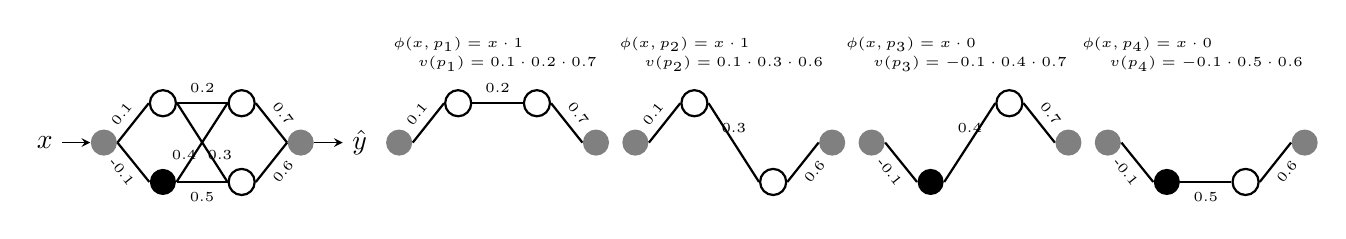
\begin{tikzpicture}
%Top Left
\node[draw,fill=white,circle,thick,
] (tl) at (-1.25,2){};

%Top Right
\node[draw,fill=white,circle,thick,
] (tr) at (-0.25,2){};

%Bottom Left
\node[fill=black,circle,
] (bl) at (-1.25,1){};

%Bottom Right
\node[draw,fill=white,circle,thick,
] (br) at (-0.25,1){};


%Input
\node[fill=gray,circle,
] (input) at (-2,1.5){};

\node[] (x) at (-2.75,1.5){$x$};


%Output
\node[fill=gray,circle,] (output) at (0.5,1.5){};

\node[] (y) at (1.25,1.5){$\hat{y}$};
\draw[-stealth](x.east)--(input.west);
\draw[-stealth](output.east)--(y.west);

\draw[-, thick] (input.east) -- (tl.west) node [midway, above, sloped] (t1) {\tiny{0.1}};
\draw[-, thick] (input.east) -- (bl.west) node [midway, below, sloped] (t2) {\tiny{-0.1}};
\draw[-, thick] (tl.east) -- (tr.west) node [midway, above, sloped] (t1) {\tiny{0.2}};
\draw[-, thick] (bl.east) -- (br.west) node [midway, below, sloped] (t1) {\tiny{0.5}};
\draw[-, thick] (tl.east) -- (br.west) node [pos=0.85, above] (t1) {\tiny{0.3}};
\draw[-, thick] (bl.east) -- (tr.west) node [pos=0.15, above] (t1) {\tiny{0.4}};
\draw[-, thick] (tr.east) -- (output.west) node [midway, above, sloped] (t1) {\tiny{0.7}};
\draw[-, thick] (br.east) -- (output.west) node [midway, below, sloped] (t1) {\tiny{0.6}};




%%%%%%%%%%%%%%%%%Path 1%%%%%%%%%%%%%%
%Input
\node[fill=gray,circle,
] (p1input) at (1.75,1.5){};


%Output
\node[fill=gray,circle,
] (p1output) at (4.25,1.5){};



%Top Left
\node[draw,fill=white,circle,thick,
] (p1tl) at (2.5,2){};

%Top Right
\node[draw,fill=white,circle,thick,
] (p1tr) at (3.5,2){};




\draw[-, thick] (p1input.east) -- (p1tl.west) node [midway, above, sloped] (t1) {\tiny{0.1}};
\draw[-, thick] (p1tl.east) -- (p1tr.west) node [midway, above, sloped] (t1) {\tiny{0.2}};
\draw[-, thick] (p1tr.east) -- (p1output.west) node [midway, above, sloped] (t1) {\tiny{0.7}};



%%%%%%%%%%%%%%%%%Path 2%%%%%%%%%%%%%%

%Input
\node[fill=gray,circle,
] (p2input) at (4.75,1.5){};


%Output
\node[fill=gray,circle,
] (p2output) at (7.25,1.5){};

%Top Left
\node[draw,fill=white,circle,thick,
] (p2tl) at (5.5,2){};

%Bottom Right
\node[draw,fill=white,circle,thick,
] (p2br) at (6.5,1){};

\draw[-, thick] (p2input.east) -- (p2tl.west) node [midway, above, sloped] (t1) {\tiny{0.1}};
\draw[-, thick] (p2tl.east) -- (p2br.west) node [pos=0.5, above] (t1) {\tiny{0.3}};
\draw[-, thick] (p2br.east) -- (p2output.west) node [midway, below, sloped] (t1) {\tiny{0.6}};



%%%%%%%%%%%%%%%%%Path 3%%%%%%%%%%%%%%

%Input
\node[fill=gray,circle,
] (p3input) at (7.75,1.5){};


%Output
\node[fill=gray,circle,
] (p3output) at (10.25,1.5){};


%Top Right
\node[draw,fill=white,circle,thick,
] (p3tr) at (9.5,2){};

%Bottom Left
\node[fill=black,circle,
] (p3bl) at (8.5,1){};



\draw[-, thick] (p3input.east) -- (p3bl.west) node [midway, below, sloped] (t2) {\tiny{-0.1}};
\draw[-, thick] (p3bl.east) -- (p3tr.west) node [pos=0.5, above] (t1) {\tiny{0.4}};
\draw[-, thick] (p3tr.east) -- (p3output.west) node [midway, above, sloped] (t1) {\tiny{0.7}};


%%%%%%%%%%%%%%%%%Path 4%%%%%%%%%%%%%%

%Input
\node[fill=gray,circle,
] (p4input) at (10.75,1.5){};


%Output
\node[fill=gray,circle,
] (p4output) at (13.25,1.5){};

%Bottom Left
\node[fill=black,circle,
] (p4bl) at (11.5,1){};

%Bottom Right
\node[draw,fill=white,circle,thick,
] (p4br) at (12.5,1){};

\draw[-, thick] (p4input.east) -- (p4bl.west) node [midway, below, sloped] (t2) {\tiny{-0.1}};
\draw[-, thick] (p4bl.east) -- (p4br.west) node [midway, below, sloped] (t1) {\tiny{0.5}};
\draw[-, thick] (p4br.east) -- (p4output.west) node [midway, below, sloped] (t1) {\tiny{0.6}};
%%%%%%%%%%%%%%%%%%%%%%%%%%%%%%

\node[] () at (2.5,2.75){\tiny{$\phi(x,p_1)=x\cdot 1$}};
\node[] () at (3.125,2.5){\tiny{$v(p_1)= 0.1 \cdot 0.2 \cdot 0.7$}};

\node[] () at (5.375,2.75){\tiny{$\phi(x,p_2)=x\cdot 1$}};
\node[] () at (6.0,2.5){\tiny{$v(p_2)=0.1 \cdot 0.3 \cdot 0.6$}};

\node[] () at (8.25,2.75){\tiny{$\phi(x,p_3)=x\cdot 0$}};
\node[] () at (9.0,2.5){\tiny{$v(p_3)= -0.1 \cdot 0.4 \cdot 0.7$}};

\node[] () at (11.25,2.75){\tiny{$\phi(x,p_4)=x\cdot 0$}};
\node[] () at (12.0,2.5){\tiny{$v(p_4)=  -0.1 \cdot 0.5 \cdot 0.6$}};




\end{tikzpicture}

